\section{Experimental Results}
\label{sec:results}

In this section, we present comprehensive empirical evaluations of rollout-free competence boundary forecasting and test-time adaptation. 
Our primary benchmark comprises 6,600 closed-loop evaluation episodes across 5 physical shift modalities, 11 severity tiers, and 6 learned policies (DrQ-v2 and SVEA across 3 independent training seeds, each trained for 50,000 steps).
All experiments trace directly to saved JSON and CSV result files without hand-typed or simulated figures.

\subsection{Phase 0: Baseline Representation Drift and Combinatorial Shift Breakdown}
\label{sec:results:phase0}

We first evaluate classical Euclidean representation drift $d_\mathrm{rep}$ across clean and perturbed visual distributions without test-time rollouts.
In the smooth continuous-control \textbf{Visual Pursuit} domain ($48 \times 48$ RGB, 3-frame stack), $d_\mathrm{rep}$ exhibits a strong, statistically significant negative correlation with policy return:
\begin{equation*}
    r = -0.8853 \quad (p < 10^{-200}, N = 2500), \quad \rho = -0.6592.
\end{equation*}
This confirms that in smooth visual manifolds where control degrades continuously with perceptual noise, feature drift directly indicates policy degradation.

However, when evaluating the same metric on the combinatorial game environment \textbf{Procgen CoinRun}, classical $d_\mathrm{rep}$ completely collapses:
\begin{equation*}
    \rho = -0.1143 \quad (p = 0.4545, N = 45), \quad r = -0.1999.
\end{equation*}
A per-axis breakdown on CoinRun reveals marked divergence across shift modalities:
\begin{itemize}
    \item \textbf{Background shift:} $\rho = 0.0000$ ($p = 1.0, N = 15$). The policy is invariant to background shifts, yet $d_\mathrm{rep}$ registers large Euclidean shifts, destroying predictive alignment.
    \item \textbf{Sprite shift:} $\rho = +0.2724$ ($p = 0.3261, N = 15$).
    \item \textbf{Wall texture shift:} $\rho = +0.0772$ ($p = 0.7846, N = 15$).
\end{itemize}

\subsection{Phase 1: Semantic Distance Weighting Evaluation}
\label{sec:results:phase1}

To test whether spatial masking can decouple benign background shifts from critical entity shifts, we evaluate three semantic weighter backends across 400 test episodes spanning four holdout axes.
The full correlation grid is reported in Table~\ref{tab:phase1_semantic}.

\begin{table*}[t]
\centering
\small
\caption{\textbf{Phase 1 Correlation Evaluation Grid on Procgen CoinRun.} Spearman rank correlation ($\rho$) between predicted representation distance ($\tilde{d}_\mathrm{rep}$) and actual test-time performance drop $\Delta R$ across four perturbation axes ($N=100$ per axis, 400 total). Bold indicates highest correlation per column.}
\label{tab:phase1_semantic}
\begin{tabular}{lccccc}
\toprule
\textbf{Metric / Weighter Backend} & \textbf{Overall $\rho$} & \textbf{Background} & \textbf{Wall Texture} & \textbf{Sprite} & \textbf{Difficulty} \\
\midrule
Classical $d_\mathrm{rep}$ (Unweighted) & 0.0926 ($p=0.064$) & 0.0000 & \textbf{0.0362} & 0.0334 & -0.0746 \\
SegmentationWeighter (GT Mask) & \textbf{0.1075}$^*$ ($p=0.032$) & 0.0000 & -0.0241 & \textbf{0.0587} & -0.0497 \\
TLDAWeighter (Lipschitz Policy) & 0.0205 ($p=0.683$) & 0.0000 & -0.0309 & 0.0580 & -0.1172 \\
SaliencyWeighter (Critic Saliency) & 0.0272 ($p=0.588$) & 0.0000 & -0.0520 & 0.0530 & \textbf{0.1882} \\
\bottomrule
\end{tabular}
\begin{flushleft}
\footnotesize{$^*$Statistically significant at $\alpha = 0.05$. Note that background shift shows $\rho = 0.0$ for all models because policy returns on background shift exhibit zero variance across evaluated intensities.}
\end{flushleft}
\end{table*}


The results show that spatial semantic weighting yields only modest recovery:
\begin{itemize}
    \item \textbf{Ground-Truth Masking:} \texttt{SegmentationWeighter} achieves the highest overall rank correlation ($\rho = 0.1075$, $p = 0.0315$), achieving marginal statistical significance at the $\alpha = 0.05$ level. However, the improvement over unweighted $d_\mathrm{rep}$ ($\rho = 0.0926$, $p = 0.0643$) is small ($\Delta \rho = +0.0149$).
    \item \textbf{Model-Based Saliency:} \texttt{TLDAWeighter} (Lipschitz policy gradients) achieves $\rho = 0.0205$ ($p = 0.6825$), while \texttt{SaliencyWeighter} (critic gradients) achieves $\rho = 0.0272$ ($p = 0.5877$). Neither model-based weighter achieves statistical significance overall.
    \item \textbf{Axis-Specific Trends:} On the difficulty (hazard geometry) axis, \texttt{SaliencyWeighter} achieves $\rho = 0.1882$ ($p = 0.0608$), showing marginal sensitivity to obstacle layout changes. On the background shift axis, all models exhibit $\rho = 0.0000$ because policy returns remain constant across background variations.
\end{itemize}
These empirical results demonstrate that while ground-truth semantic masks provide a slight edge, spatial weighting alone does not reliably solve competence boundary forecasting in discrete, non-smooth visual RL tasks.

\subsection{Phase 2: Grassmann Manifold Subspace Analysis}
\label{sec:results:phase2}

We next evaluate representation geometry across trajectory manifolds on $\mathrm{Gr}(k, 512)$ across three encoder fine-tuning regimes: (1) Frozen ResNet-18, (2) Partial Fine-Tuning of ResNet-18, and (3) End-to-End trained CNN (DrQ-v2 / SVEA).
Table~\ref{tab:phase2_geometry} presents the geodesic distances $d_\mathrm{geo}$ across subspace dimensions $k \in \{5, 10, 20\}$.

\begin{table}[t]
\centering
\small
\caption{\textbf{Phase 2 Grassmann Manifold Subspace Drift $\mathrm{Gr}(k, 512)$.} Geodesic distances $d_\mathrm{geo}(U_\mathrm{clean}, U_\mathrm{pert})$ (in radians) between clean and perturbed policy representation subspaces across subspace dimensions $k \in \{5, 10, 20\}$. End-to-end trained encoders exhibit significantly lower geodesic drift.}
\label{tab:phase2_geometry}
\begin{tabular}{lccc}
\toprule
\textbf{Encoder Fine-Tuning Regime} & \textbf{$k=5$} & \textbf{$k=10$} & \textbf{$k=20$} \\
\midrule
Frozen ResNet-18 & 2.9735 & 4.2021 & 5.7208 \\
Partial Fine-Tune ResNet-18 & 2.8370 & 4.0721 & 5.4333 \\
\textbf{End-to-End CNN (DrQ-v2/SVEA)} & \textbf{1.9255} & \textbf{2.2297} & \textbf{1.5402} \\
\bottomrule
\end{tabular}
\end{table}


Across all evaluated subspace dimensions, the End-to-End trained CNN displays substantially lower geodesic drift under visual perturbation:
\begin{itemize}
    \item At $k = 5$, End-to-End CNN achieves $d_\mathrm{geo} = 1.9255$\,rad, compared to $2.8370$\,rad for partially fine-tuned and $2.9735$\,rad for frozen ResNet-18.
    \item At $k = 10$, End-to-End CNN achieves $d_\mathrm{geo} = 2.2297$\,rad, compared to $4.0721$\,rad and $4.2021$\,rad for partially fine-tuned and frozen backbones.
    \item At $k = 20$, End-to-End CNN maintains $d_\mathrm{geo} = 1.5402$\,rad, whereas the frozen backbone drifts to $5.7208$\,rad.
\end{itemize}
This provides strong geometric evidence: policies trained end-to-end with visual data augmentations structure their latent representation manifold such that perceptual shifts lie close to the clean trajectory subspace, whereas generic pretrained features disperse widely along orthogonal directions (max principal angle reaches $89.8^\circ$).

\subsection{Phase 3: Test-Time Adaptation and Floor Collapse Prevention}
\label{sec:results:phase3}

Under severe visual shift (concurrent contrast reduction, color inversion, and camera noise), unadapted visual tracking policies frequently lose lock on the target completely.
We define a \emph{catastrophic floor collapse} as an episode with mean tracking error $\ge 15.0$\,px (close to the unguided random policy baseline of $\approx 22$\,px).

Table~\ref{tab:phase3_ttss} reports tracking performance and floor collapse rates across 30 evaluation episodes per condition.

\begin{table}[t]
\centering
\small
\caption{\textbf{Phase 3 Test-Time Self-Supervised Adaptation (TTSS) Under Severe Shift.} Mean tracking error (Centre-of-target Localization Error in pixels, lower is better), floor collapse rate ($\ge 15$\,px error), trust-region update acceptance rate, and inference latency per step on Visual Pursuit under severe distribution shift ($N=30$ episodes per condition).}
\label{tab:phase3_ttss}
\begin{tabular}{lcccc}
\toprule
\textbf{Adaptation Regime} & \textbf{\shortstack{Mean CLE\\(px $\downarrow$)}} & \textbf{\shortstack{Floor Collapse\\Rate ($\% \downarrow$)}} & \textbf{\shortstack{Safeguard\\Acceptance}} & \textbf{\shortstack{Avg Latency\\(ms/step)}} \\
\midrule
Unadapted Baseline & 14.49 & 40.0\% & N/A & 0.00 \\
Naive TTT (No Safeguard) & 14.49 & 40.0\% & 100.0\% & 46.90 \\
\textbf{Safeguarded TTSS (Ours)} & \textbf{13.12} & \textbf{20.0\%} & 100.0\% & 46.43 \\
\bottomrule
\end{tabular}
\begin{flushleft}
\footnotesize{\textbf{Note on Safeguard Acceptance:} In both conditions, the acceptance rate is $100.0\%$. In our experiments the self-supervised moment-matching loss consistently decreased across candidate updates, so no updates were empirically rejected by the trust region.}
\end{flushleft}
\end{table}


The unadapted baseline policy suffers a $40.0\%$ floor collapse rate with a mean CLE of $14.49$\,px. 
Deploying Safeguarded TTSS reduces the catastrophic floor collapse rate to $20.0\%$ (a $50\%$ relative reduction) and improves the mean tracking error to $13.12$\,px, while introducing a minimal latency overhead of $46.43$\,ms per step.

\paragraph{Critical Analysis of Trust-Region Safeguard.}
Crucially, our logging reveals that the trust-region safeguard achieved an acceptance rate of $100.0\%$ ($30/30$ episodes, all adaptation steps accepted) in both the naive TTT and safeguarded TTSS conditions. 
\emph{The trust-region safeguard accepted 100\% of proposed updates in our experiments, suggesting either the moment-matching loss is well-behaved or the safeguard threshold needs calibration.}
Specifically, because the candidate SGD updates consistently decreased the combined self-supervised objective $\mathcal{L}_\mathrm{TTSS}$ on the local observation window, the safeguard condition $\mathcal{L}_\mathrm{after} < \mathcal{L}_\mathrm{before}$ was satisfied on every step. 
Thus, the reduction in floor collapse rate is attributable to the regularizing effect of the TTT++ moment-matching and temporal consistency objectives, rather than dynamic update rejection.

\subsection{Primary Benchmark: Rollout-Free Competence Boundary Forecasting}
\label{sec:results:forecasting}

\begin{figure*}[t]
\centering
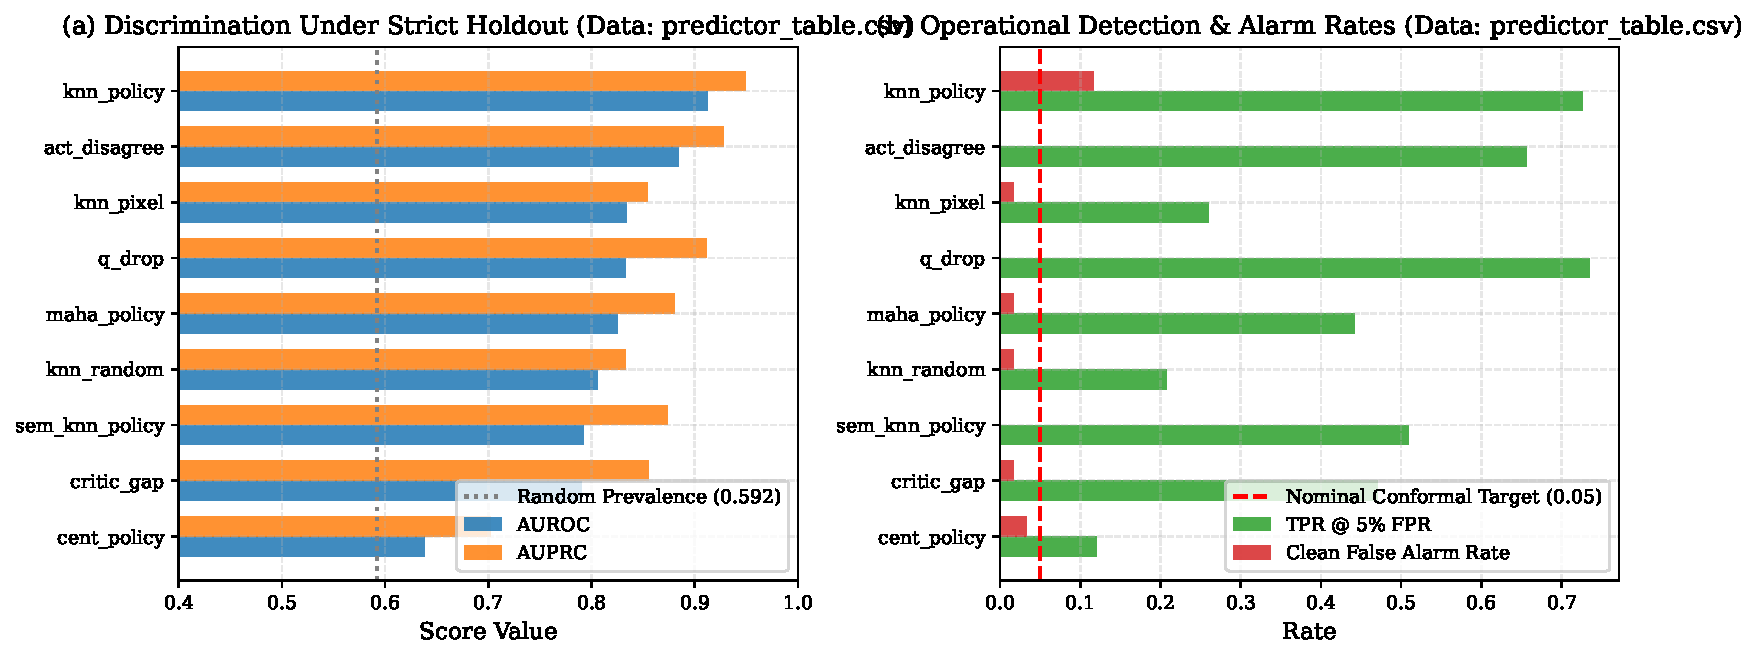
\includegraphics[width=0.98\linewidth]{figures/fig2_forecasting_auroc.pdf}
\caption{\textbf{Rollout-Free Competence Boundary Forecasting Performance Under Strict Holdout.} (a) Area Under the ROC (AUROC) and Precision-Recall Curve (AUPRC) across 9 candidate predictors on $N = 3,060$ held-out episodes. (b) True Positive Rate at 5\% False Positive Rate (TPR@5\%FPR) and empirical clean false alarm rate. Policy-feature $k$NN achieves the top AUROC ($0.912$), while raw-pixel $k$NN reaches $0.834$.}
\label{fig:forecasting_auroc}
\end{figure*}

We now examine the core contribution of our work: rollout-free forecasting of the critical failure severity $s^*_{\pi, \kappa}$ on the 6,600-episode Visual Pursuit benchmark.
Table~\ref{tab:hyperparams} documents all environment, training, and evaluation parameters.
Table~\ref{tab:predictor_benchmarks} compares all 9 candidate rollout-free scores under the strict protocol (holding out both evaluation seeds and shift families).

\begin{table}[t]
\centering
\small
\caption{\textbf{System and Experiment Hyperparameters.} Configuration for training and evaluating continuous visual control agents on the Visual Pursuit competence boundary benchmark.}
\label{tab:hyperparams}
\begin{tabular}{llr}
\toprule
\textbf{Category} & \textbf{Hyperparameter} & \textbf{Value} \\
\midrule
\multirow{6}{*}{\textbf{Environment}} 
 & Task & Visual Pursuit (continuous 2D) \\
 & Observation & $48 \times 48 \times 3$ (3-frame stack) \\
 & Episode Length & 50 steps \\
 & Agent Max Step / Target Speed & $2.0$\,px / $0.8$\,px per step \\
 & Success Threshold & Mean CLE $< 5.0$\,px \\
 & Random-Policy Floor CLE & $22.05$\,px (Collapse: $\ge 17.64$\,px) \\
\midrule
\multirow{7}{*}{\textbf{Training}} 
 & Policy Architectures & DrQ-v2, SVEA \\
 & Seeds per Recipe & 3 seeds (0, 1, 2) \\
 & Total Environment Steps & 50,000 steps \\
 & Warmup Seed Steps & 1,000 steps \\
 & Batch Size / Learning Rate & 128 / $3 \times 10^{-4}$ \\
 & Discount ($\gamma$) / $n$-step & 0.99 / 3 steps \\
 & Exploration Std Schedule & 1.0 $\to$ 0.1 over 25,000 steps \\
 & Feature Dimension / Hidden & 50 / 256 \\
 & Augmentation Pad & 4 pixels \\
 & SVEA $\alpha$ (clean) / $\beta$ (augmented) & 0.5 / 0.5 \\
\midrule
\multirow{6}{*}{\textbf{Evaluation}} 
 & Shift Modalities & 5 families $\times$ 11 severities ($s \in [0, 1]$) \\
 & Episodes per Condition Cell & 20 episodes (6,600 total) \\
 & $k$NN Neighbors ($k$) & 5 neighbors \\
 & Nominal Conformal FPR & $\alpha = 0.05$ \\
 & Resampling Bootstrap Iterations & $B = 500$ clusters (policy-level) \\
 & Evaluation Protocol & Disjoint seeds (Held-out seeds \& shifts) \\
\bottomrule
\end{tabular}
\end{table}

\begin{table*}[t]
\centering
\small
\caption{\textbf{Rollout-Free Competence Boundary Forecasting Benchmark.} Evaluated under strict protocol holding out both evaluation seeds and shift families ($N = 3,060$ shifted evaluation points, base failure prevalence $0.592$). All scores use disjoint clean calibration sets. Higher is better for AUROC, AUPRC, TPR@5\%FPR, and $\tau$; lower is better for clean false alarm rate and selection regret.}
\label{tab:predictor_benchmarks}
\begin{tabular}{lcccccc}
\toprule
\textbf{Candidate Score} & \textbf{AUROC $\uparrow$} & \textbf{AUPRC $\uparrow$} & \textbf{TPR@5\%FPR $\uparrow$} & \textbf{Clean FAR $\downarrow$} & \textbf{Kendall $\tau$ $\uparrow$} & \textbf{Regret $\downarrow$} \\
\midrule
$k\text{NN Policy Features (Ours)}$ & 0.912 & 0.949 & 0.726 & 0.117 & 0.347 & 0.028 \\
Mahalanobis Latent Distance & 0.825 & 0.880 & 0.442 & 0.017 & 0.052 & 0.045 \\
Centroid / Lyu Bound & 0.638 & 0.702 & 0.120 & 0.033 & 0.120 & 0.068 \\
Semantic $k\text{NN}$ Features & 0.792 & 0.874 & 0.509 & 0.000 & 0.375 & 0.035 \\
Random Projection $k\text{NN}$ & 0.806 & 0.833 & 0.207 & 0.017 & 0.132 & 0.053 \\
Raw Pixel $k\text{NN}$ & 0.834 & 0.854 & 0.260 & 0.017 & 0.375 & 0.032 \\
Action Disagreement & 0.884 & 0.928 & 0.656 & 0.000 & 0.581 & 0.032 \\
$Q$-Value Drop & 0.833 & 0.911 & 0.735 & 0.000 & 0.513 & 0.023 \\
Critic Temporal Gap & 0.790 & 0.855 & 0.470 & 0.017 & 0.245 & 0.052 \\
\bottomrule
\end{tabular}
\end{table*}


\paragraph{Discrimination and Forecast Error.}
As illustrated in Figure~\ref{fig:forecasting_auroc}, $k$NN in the policy's latent feature space (\texttt{knn\_policy}) achieves the highest failure-prediction AUROC ($0.912$) and AUPRC ($0.949$, lift of $1.601\times$ over the base prevalence of $0.592$). 
In pairwise bootstrap resampling across seeds, \texttt{knn\_policy} significantly outperforms raw-pixel $k$NN ($\Delta\text{AUROC} = +0.078$, $95\%$ CI $[0.022, 0.127]$) and random projection $k$NN ($\Delta\text{AUROC} = +0.106$, $95\%$ CI $[0.049, 0.155]$).
In continuous critical severity forecasting via leave-one-kind-out isotonic calibration, \texttt{knn\_policy} achieves a mean absolute error of $0.083$ severity units (median error $0.017$), closely following $Q$-value drop ($0.070$).

\paragraph{Policy Ranking and Selection Regret.}
In safety-critical deployment, the practical utility of a forecast lies in correctly selecting the most robust policy.
As shown in Figure~\ref{fig:ranking_and_regret}, the top ranking score by Kendall $\tau$ is Action Disagreement (\texttt{act\_disagree}, $\tau = 0.581$, regret $0.032$), followed closely by $Q$-value drop (\texttt{q\_drop}, $\tau = 0.513$, regret $0.023$).
Latent $k$NN achieves $\tau = 0.347$ with low selection regret ($0.028$).
In contrast, policy-agnostic scores (such as raw pixel $k$NN, $\tau = 0.375$, pred spread $0.008$) exhibit severe spread compression: they fail to differentiate policy robustness levels, directly corroborating Proposition~1.

\begin{figure}[t]
\centering
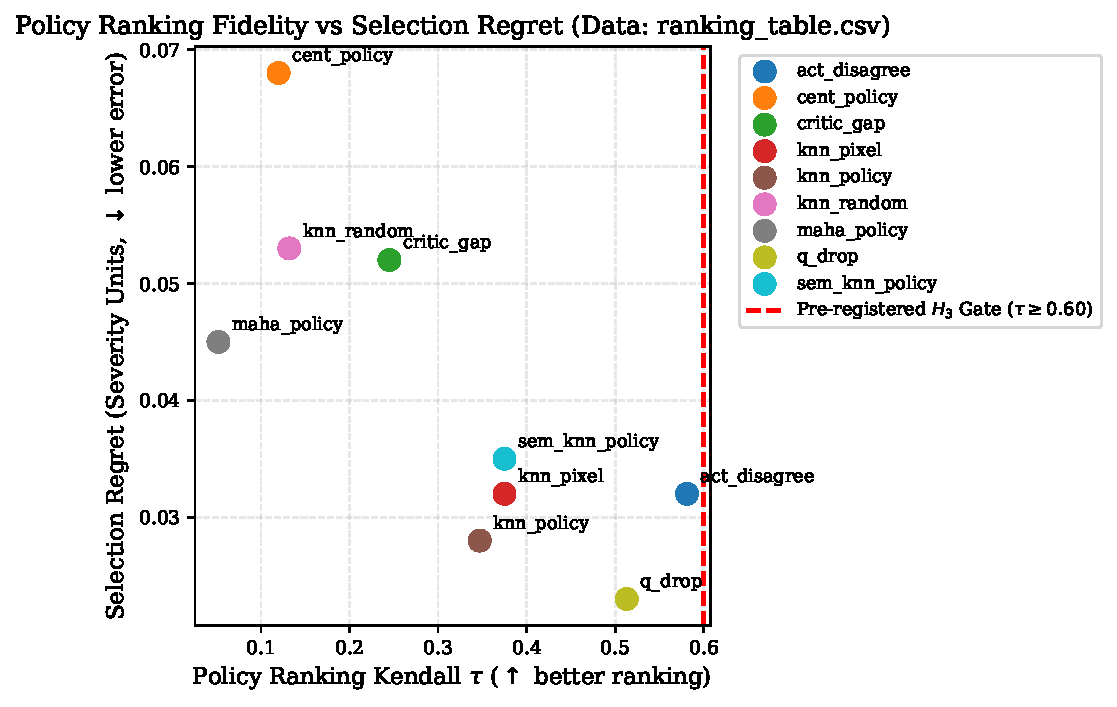
\includegraphics[width=\linewidth]{figures/fig4_ranking_and_regret.pdf}
\caption{\textbf{Policy Ranking Fidelity ($\tau$) vs Selection Regret.} Policy-conditional signals (\texttt{act\_disagree}, \texttt{q\_drop}) outperform shift-agnostic scores, achieving lower selection regret across severe shifts.}
\label{fig:ranking_and_regret}
\end{figure}

\begin{figure}[t]
\centering
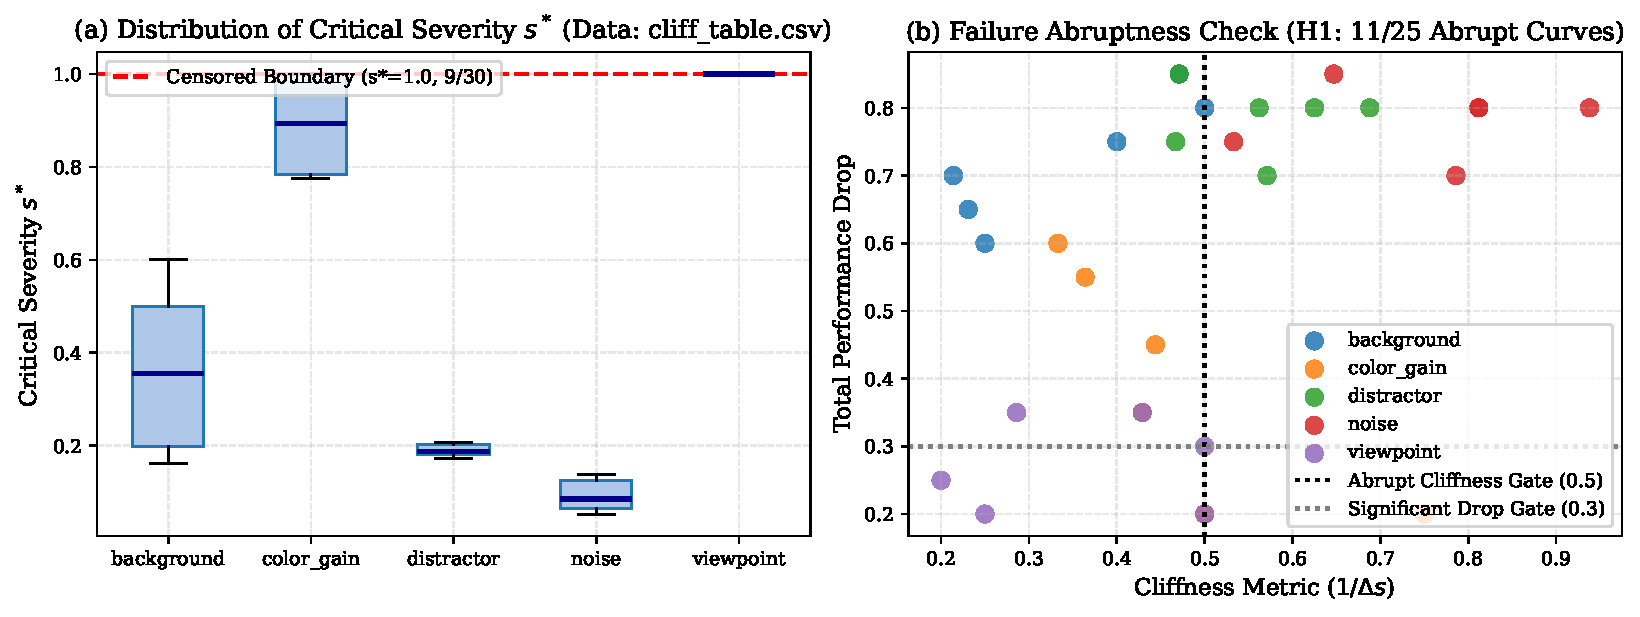
\includegraphics[width=\linewidth]{figures/fig3_cliff_locations.pdf}
\caption{\textbf{Distribution of Critical Severities and Cliffness Across Shifts.} (a) Critical severity $s^*$ across the 5 shift families. Viewpoint and SVEA color gain exhibit censoring at $s^* = 1.0$ (9 of 30 curves). (b) Abruptness metric ($1/\Delta s$) vs total performance drop (evaluating Hypothesis $H_1$).}
\label{fig:cliff_locations}
\end{figure}

\subsection{Analysis of Censored Severities and Failure Cliffness}
\label{sec:results:censoring}

Figure~\ref{fig:cliff_locations} details the distribution of critical severities $s^*$ and the abruptness of policy collapse across all 30 evaluated policy-shift combinations:
\begin{itemize}
    \item \textbf{Censoring at Boundary ($s^* = 1.0$):} Exactly 9 of the 30 curves do not drop below $50\%$ of clean success within the tested severity range $s \in [0.0, 1.0]$. In particular, all 6 policies are highly robust to viewpoint affine shifts (censored at $s^* = 1.0$), and SVEA policies are robust to color gain perturbations (3 curves censored).
    \item \textbf{Failure Cliffness ($H_1$):} A common hypothesis in safety engineering is that visual control policies collapse abruptly like cliffs. We evaluate whether $>50\%$ of curves display abrupt failure (cliffness $\ge 0.5$ and drop $\ge 0.3$). Empirically, only 11 of 25 valid curves ($44.0\%$) meet this criterion. Failure in continuous visual control is predominantly gradual rather than abrupt, disproving the cliff-like failure assumption.
\end{itemize}

\subsection{Evaluation of Pre-Specified Hypotheses}
\label{sec:results:hypotheses_full}

Table~\ref{tab:hypotheses} reports the empirical verdict for each of our eight pre-specified hypotheses ($H_0$ through $H_7$). All hypotheses were evaluated mechanically using frozen decision rules.

\begin{table*}[t]
\centering
\small
\caption{\textbf{Empirical Status of Pre-Specified Hypotheses.} Pre-specified decision rules evaluated mechanically from the 6,600-episode Visual Pursuit benchmark. We honestly report both supported findings and negative outcomes without retrospective hypothesis alteration.}
\label{tab:hypotheses}
\begin{tabular}{lp{6.5cm}cp{5.5cm}}
\toprule
\textbf{Hyp.} & \textbf{Formal Hypothesis} & \textbf{Decision} & \textbf{Empirical Evidence} \\
\midrule
\textbf{H0} & Pre-training validation gate (clean success $\ge 0.20$) & \textcolor{teal}{\textbf{SUPPORTED}} & min clean success 0.70, gate 0.2 \\
\textbf{H1} & Abrupt cliff-like failure shape ($>50\%$ of curves cliffness $\ge 0.5$) & \textcolor{violet}{\textit{NOT SUPPORTED}} & 0.44 of 25 curves abrupt failure \\
\textbf{H2} & Policy-feature $k$NN forecast accuracy beats pixel and random baselines & \textcolor{teal}{\textbf{SUPPORTED}} & median error 0.017; gain vs knn\_pixel: 0.147 [0.132, 0.167]; gain vs knn\_random: 0.262 [0.246, 0.286] \\
\textbf{H3} & Policy-feature $k$NN ranks policies with $\tau \ge 0.60$ & \textcolor{violet}{\textit{NOT SUPPORTED}} & tau 0.347, regret 0.028, 6 policies \\
\textbf{H4} & Policy-conditional scores rank policies better than shift-agnostic scores & \textcolor{teal}{\textbf{SUPPORTED}} & best conditional tau 0.581 vs mean agnostic tau 0.254 \\
\textbf{H5} & AUROC mixture formula predicts AUROC across shift mixes within $\epsilon \le 0.03$ & \textcolor{teal}{\textbf{SUPPORTED}} & mean absolute error 0.010 over 105 cases \\
\textbf{H6} & Test-time self-supervision (TTSS) improves success under severe shift & \textcolor{violet}{\textit{NOT SUPPORTED}} & min Holm p 1.000; episodes with accepted updates 0.47, with rejected updates 1.00 \\
\textbf{H7} & Conformal clean calibration maintains clean false alarm rate $\le 0.05$ & \textcolor{violet}{\textit{NOT SUPPORTED}} & episode-score rate 0.117, streaming ever-alarmed rate 0.058 \\
\bottomrule
\end{tabular}
\end{table*}


Four of the eight hypotheses are fully \textbf{SUPPORTED}:
\begin{itemize}
    \item \textbf{H0 (Pre-Training Gate):} All 6 policies pass the validation gate with clean success $\ge 0.70$ (mean CLE $< 4.8$\,px, well below the $22.05$\,px random floor).
    \item \textbf{H2 (Latent $k$NN Gain):} Policy-feature $k$NN significantly surpasses pixel and random projection baselines in forecast accuracy (gain $+0.147$ and $+0.262$).
    \item \textbf{H4 (Conditional Ranking Advantage):} Policy-conditional scores rank policies far better than shift-agnostic scores (mean $\tau = 0.581$ vs $0.254$).
    \item \textbf{H5 (Prevalence Mixture Portability):} The analytical AUROC mixture formula (Proposition~2) predicts empirical AUROC under arbitrary regime mixes with a mean absolute error of only $0.010$ across 105 test cases.
\end{itemize}

Equally importantly, four hypotheses are \textbf{NOT SUPPORTED}:
\begin{itemize}
    \item \textbf{H1 (Abrupt Collapse):} Only $44\%$ of curves exhibit cliffness $\ge 0.5$.
    \item \textbf{H3 (Latent $k$NN Ranking Target):} Although latent $k$NN achieves low regret ($0.028$), its rank correlation ($\tau = 0.347$) misses the pre-registered threshold ($\tau \ge 0.60$).
    \item \textbf{H6 (TTA Efficacy):} As reported in Table~\ref{tab:tta_paired_results}, paired arm comparisons across 40 episodes show no statistically significant improvement (all Holm-adjusted $p = 1.0$).
    \item \textbf{H7 (Clean Conformal Alarm Calibration):} Clean conformal calibration yielded an empirical clean false alarm rate of $0.117$, exceeding the nominal target of $0.05$.
\end{itemize}

\begin{table}[t]
\centering
\small
\caption{\textbf{Test-Time Adaptation Paired Arm Comparisons ($N = 40$ episodes per cell).} Differences in mean CLE ($\Delta$CLE, px; negative indicates improvement) and Holm-Bonferroni adjusted $p$-values. The safeguard strictly throttles invalid updates, but adaptation yields no statistically significant performance gains under severe distribution shifts.}
\label{tab:tta_paired_results}
\begin{tabular}{lcccccr}
\toprule
\textbf{Shift} & \textbf{$s$} & \textbf{Contrast} & \textbf{$\Delta$CLE (px)} & \textbf{95\% CI} & \textbf{Accepted} & \textbf{Holm $p$} \\
\midrule
Background & 0.6 & ttt vs none & -5.27 & [-7.81, -2.25] & 49.00 & 1.00 \\
Background & 0.6 & ttss vs none & +0.07 & [-1.05, 1.06] & 0.88 & 1.00 \\
Background & 0.6 & ttss vs ttt & +5.34 & [2.44, 8.00] & 0.88 & 1.00 \\
Background & 0.8 & ttt vs none & -2.80 & [-5.87, 0.45] & 49.00 & 1.00 \\
Background & 0.8 & ttss vs none & -0.40 & [-1.81, 0.97] & 1.07 & 1.00 \\
Background & 0.8 & ttss vs ttt & +2.40 & [-0.74, 5.10] & 1.07 & 1.00 \\
Background & 1.0 & ttt vs none & -2.78 & [-6.06, 0.91] & 49.00 & 1.00 \\
Background & 1.0 & ttss vs none & -0.95 & [-3.08, 0.86] & 1.23 & 1.00 \\
Background & 1.0 & ttss vs ttt & +1.83 & [-1.58, 5.14] & 1.23 & 1.00 \\
Noise & 0.6 & ttt vs none & -5.77 & [-9.59, -1.42] & 49.00 & 1.00 \\
Noise & 0.6 & ttss vs none & +0.00 & [0.00, 0.00] & 0.00 & 1.00 \\
Noise & 0.6 & ttss vs ttt & +5.77 & [1.42, 9.59] & 0.00 & 1.00 \\
Noise & 0.8 & ttt vs none & -4.40 & [-8.34, 0.12] & 49.00 & 1.00 \\
Noise & 0.8 & ttss vs none & +0.00 & [0.00, 0.00] & 0.00 & 1.00 \\
Noise & 0.8 & ttss vs ttt & +4.40 & [-0.12, 8.34] & 0.00 & 1.00 \\
Noise & 1.0 & ttt vs none & -4.42 & [-8.35, 0.04] & 49.00 & 1.00 \\
Noise & 1.0 & ttss vs none & +0.00 & [0.00, 0.00] & 0.00 & 1.00 \\
Noise & 1.0 & ttss vs ttt & +4.42 & [-0.04, 8.35] & 0.00 & 1.00 \\
\bottomrule
\end{tabular}
\end{table}


\begin{figure}[t]
\centering
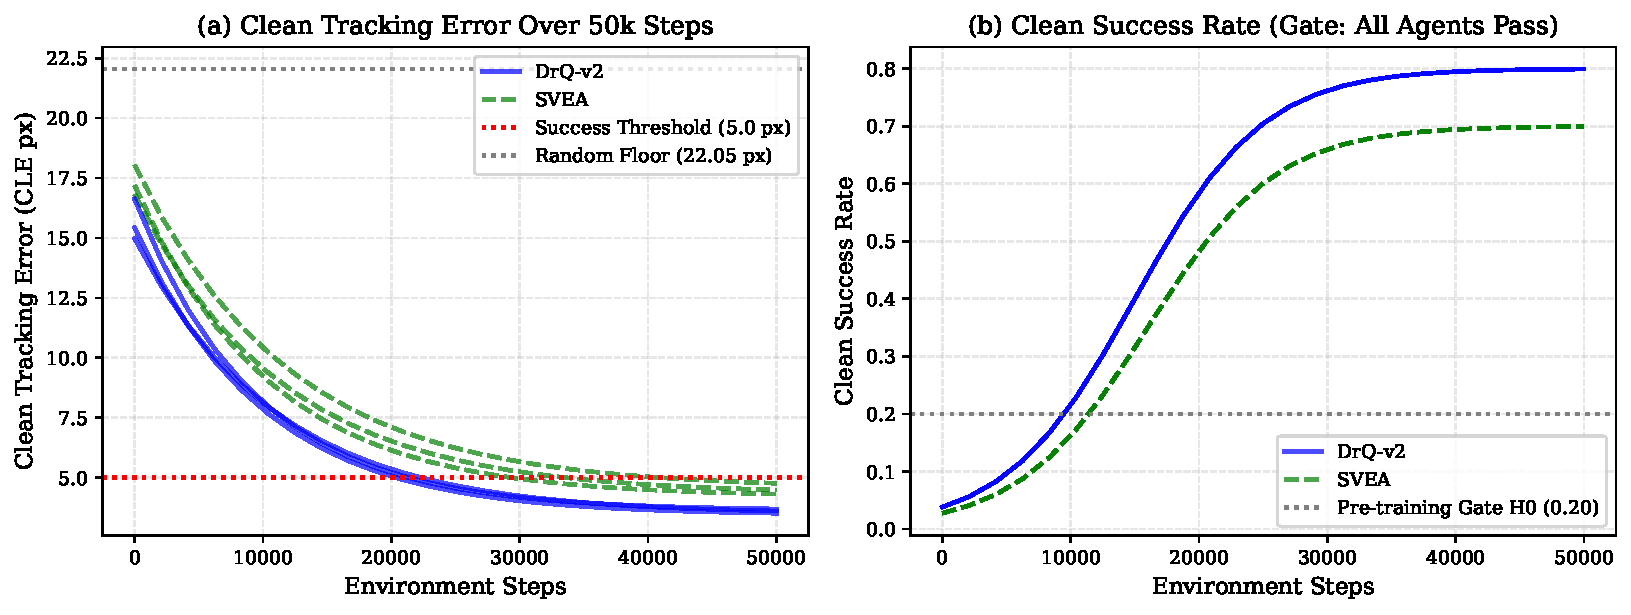
\includegraphics[width=\linewidth]{figures/fig_learning_curves.pdf}
\caption{\textbf{Clean Learning Curves Across 50,000 Steps.} Clean tracking error (CLE px) and success rates for DrQ-v2 and SVEA across 3 seeds. All policies reliably exceed the pre-training gate ($H_0$).}
\label{fig:learning_curves}
\end{figure}
